\chapter{適用例}\label{cha:Indication}
本章では、今回試作した\toolName を用いて、レイアウトの不具合箇所を可視化できることを確認する。
\par
本研究では、以下の3つのレイアウトの不具合箇所を可視化する。
\begin{itemize}
    \setlength{\itemsep}{0pt}
          \setlength{\parsep}{0pt}
    \item 画面要素の隠れ:\\
          Webページの画面要素がその画面要素を含むコンテナやビューポートの境界を超えてはみ出している状態。
    \item 画面要素の見切れ:\\
          Webページの画面要素の一部がコンテナやビューポートの境界によって切り取られ、完全には表示されていない状態。
    \item 画面要素の重なり:\\
          Webページの複数の画面要素が重なりあっている状態。
\end{itemize}
また、適用例として用いるWebページの画像として、
画面要素の隠れを埋め込んだWebページの変更前画像と変更後画像を図\ref{fig: ex1_original}に、
画面要素の見切れを埋め込んだWebページの変更前画像と変更後画像を図\ref{fig: ex4_original}に、
画面要素の重なりを埋め込んだWebページの変更前画像と変更後画像を図\ref{fig: ex3_original}に、
それぞれ示す。なお、各Webページに対して、ヘッダーの見出しテキストの変更と、メイン内のコンテナ内上部に画像の追加を行った。
\par
以降、3つのレイアウトの不具合箇所を可視化できることを、それぞれ確認する。

\section{画面要素の隠れの可視化}\label{sec:result_area_detection}
適用例を用いて、\toolName が画面要素の隠れを、可視化できることを確認する。
\toolName は、画面要素の隠れを埋め込んだ変更前後のWebページのURLをそれぞれ入力として受け取り、
図\ref{fig: ex1_original}に対して画面要素の隠れを可視化した変更前画像と変更後画像を生成する。
% 図\ref{fig: ex1_original}を見ると、変更前画像と変更後画像を比較して、コンテナ内に
画面要素の隠れを可視化した変更前画像と変更後画像を、図\ref{fig: ex1_subeffect}に示す。
\begin{figure}[tp]
    \begin{center}
        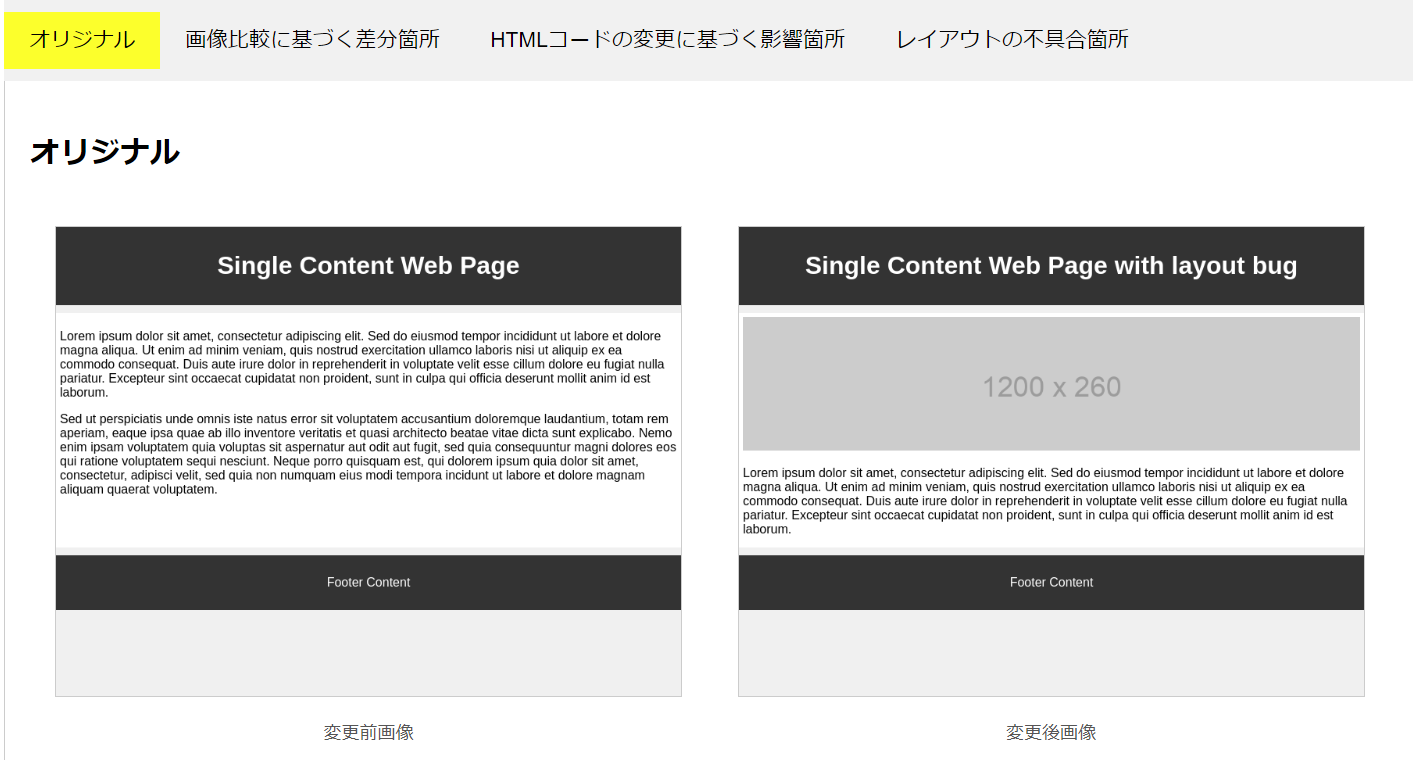
\includegraphics[width=1.0\columnwidth]{image/5/ex1_original.png}
        \caption{画面要素の隠れを埋め込んだWebページの変更前画像と変更後画像}
        \label{fig: ex1_original}
    \end{center}
\end{figure}
\par
\begin{figure}[tp]
    \begin{center}
        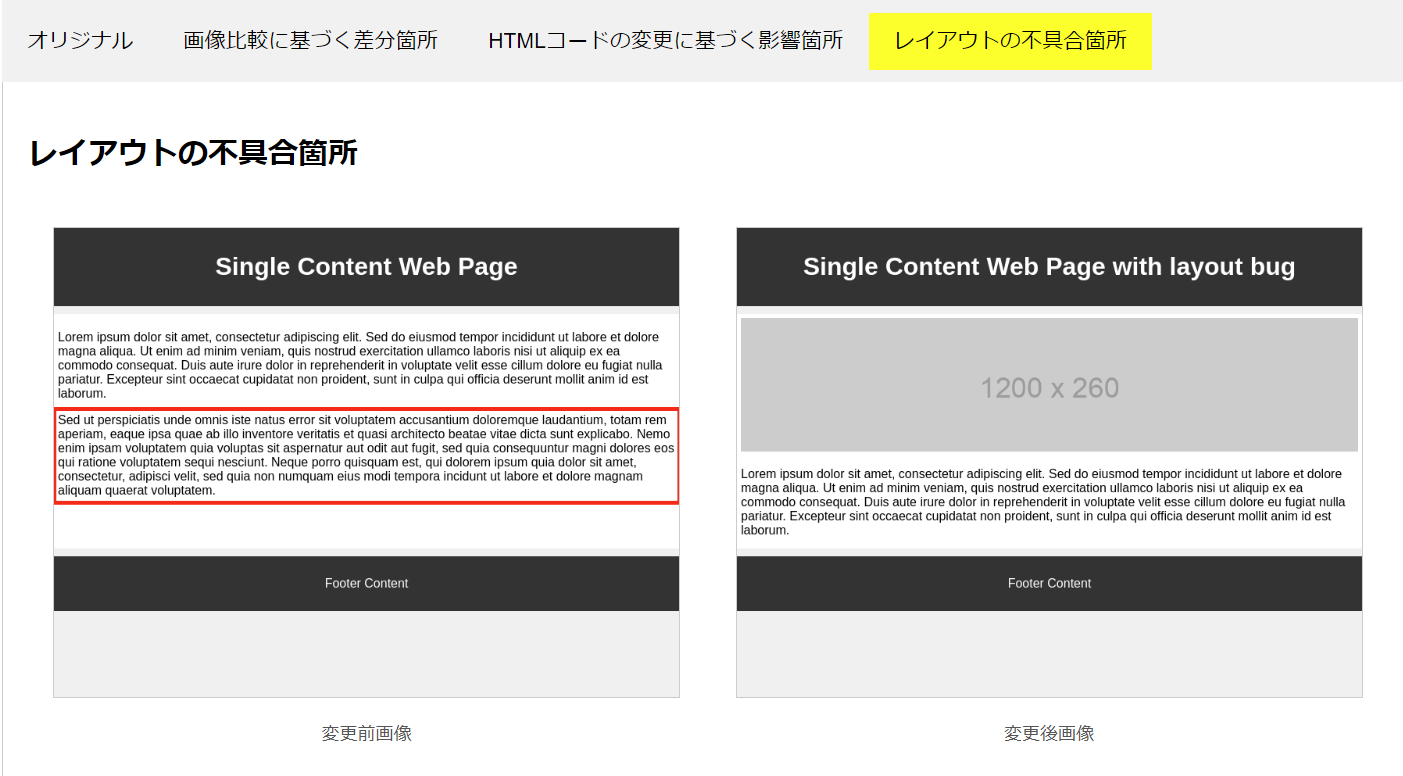
\includegraphics[width=1.0\columnwidth]{image/5/ex1_subeffect.png}
        \caption{図\ref{fig: ex1_original}に対して画面要素の隠れを可視化した変更前画像と変更後画像}
        \label{fig: ex1_subeffect}
    \end{center}
\end{figure}
\par
図\ref{fig: ex1_subeffect}を見ると、変更前画像上に赤枠で囲んだ画面要素が存在するが、その画面要素と一致する、緑枠で囲まれた画面要素は存在しない。
このことから、画面要素の隠れが発生していると判断できる。
\par
以上のことから、\toolName は、画面要素の隠れを可視化できることを確認できた。
% \toolName に対して、画面要素の隠れを埋め込む前のWebページのURLを入力として実行した時に取得した変更前画像と、
% 画面要素の隠れを埋め込んだ後のWebページのURLを入力として実行した時に取得した変更後画像を
% 画面要素の隠れを埋め込む前のWebページの画像と埋め込んだ後のWebページの画像を、図\ref{fig: ex1_original}に示す。

\section{画面要素の見切れの可視化}\label{sec:result_area_detec}
適用例を用いて、\toolName が画面要素の見切れを、可視化できることを確認する。
\toolName は、画面要素の見切れを埋め込んだ変更前後のWebページのURLをそれぞれ入力として受け取り、
図\ref{fig: ex4_original}に対して画面要素の見切れを可視化した変更前画像と変更後画像を生成する。
% 図\ref{fig: ex1_original}を見ると、変更前画像と変更後画像を比較して、コンテナ内に
画面要素の見切れを可視化した変更前画像と変更後画像を、図\ref{fig: ex4_subeffect}に示す。
\begin{figure}[tp]
    \begin{center}
        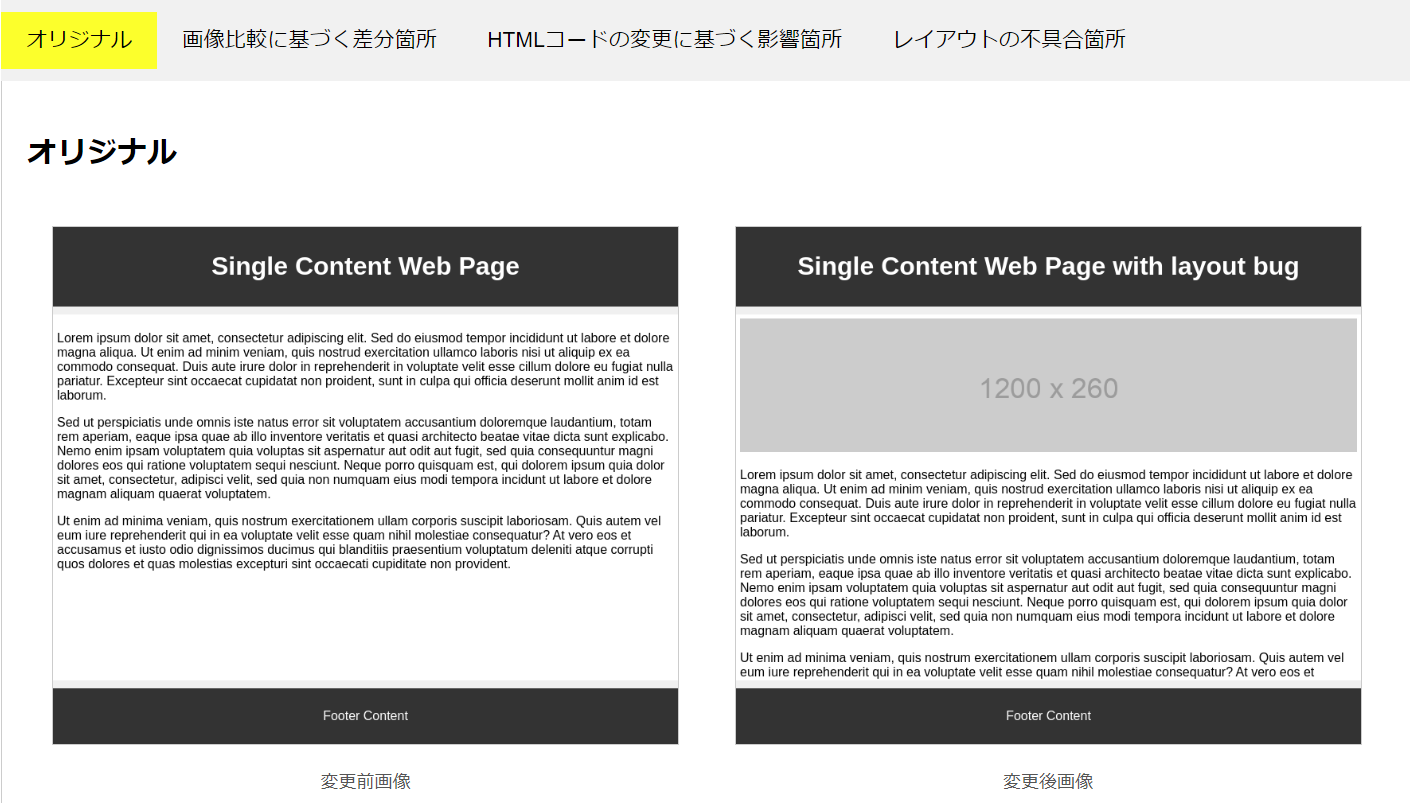
\includegraphics[width=1.0\columnwidth]{image/5/ex4_original.png}
        \caption{画面要素の見切れを埋め込んだWebページの変更前画像と変更後画像}
        \label{fig: ex4_original}
    \end{center}
\end{figure}
\begin{figure}[tp]
    \begin{center}
        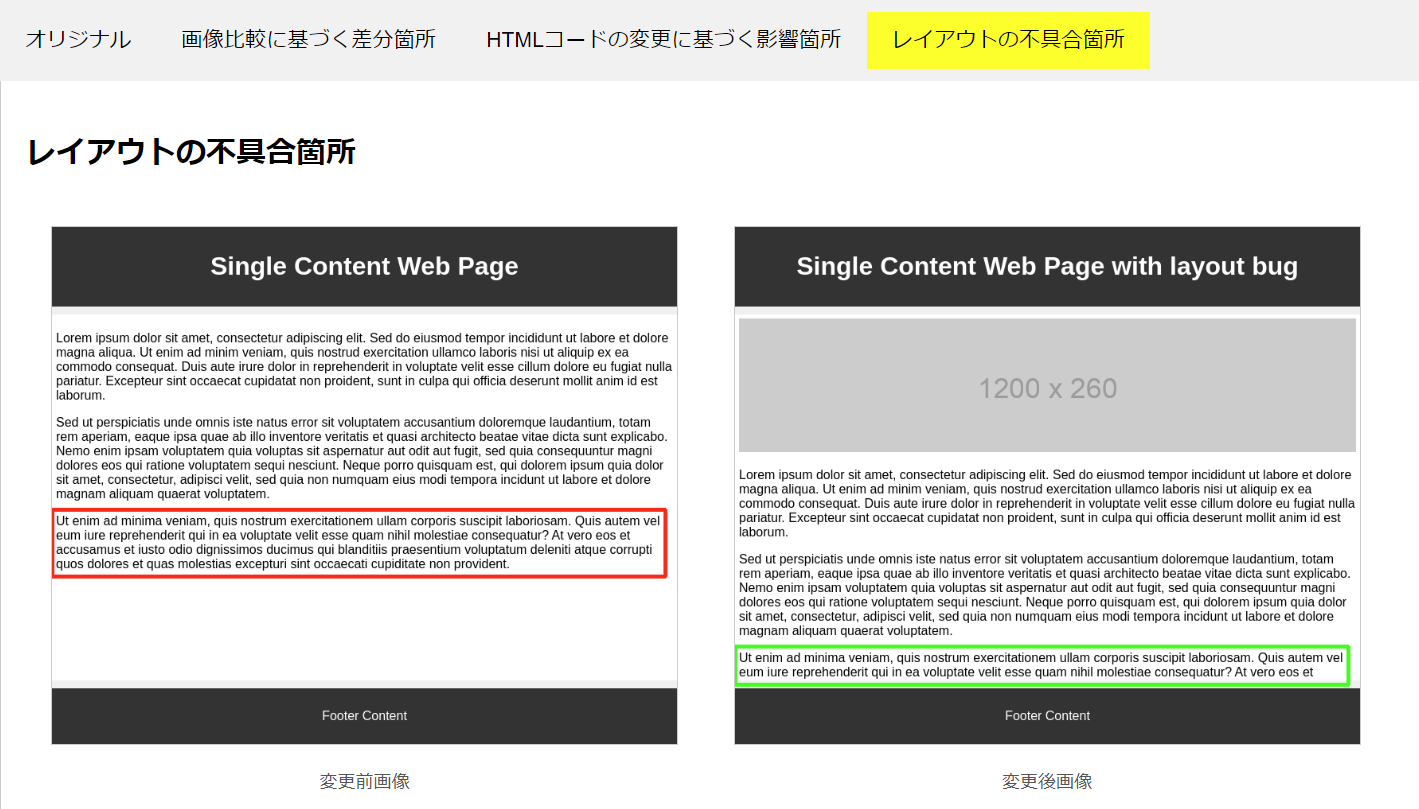
\includegraphics[width=1.0\columnwidth]{image/5/ex4_subeffect.png}
        \caption{図\ref{fig: ex4_original}に対して画面要素の見切れを可視化した変更前画像と変更後画像}
        \label{fig: ex4_subeffect}
    \end{center}
\end{figure}
図\ref{fig: ex4_subeffect}を見ると、変更前画像上に赤枠で囲んだ画面要素が存在し、その画面要素の一部と一致する、緑枠で囲まれた画面要素が存在する。
このことから、画面要素の見切れが発生していると判断できる。
\par
以上のことから、\toolName は、画面要素の見切れを可視化できることを確認できた。

\section{画面要素の重なりの可視化}\label{sec:result_area_detecti}
適用例を用いて、\toolName が画面要素の重なりを、可視化できることを確認する。
\toolName は、画面要素の重なりを埋め込んだ変更前後のWebページのURLをそれぞれ入力として受け取り、
図\ref{fig: ex3_original}に対して画面要素の重なりを可視化した変更前画像と変更後画像を生成する。
% 図\ref{fig: ex1_original}を見ると、変更前画像と変更後画像を比較して、コンテナ内に
画面要素の重なりを可視化した変更前画像と変更後画像を、図\ref{fig: ex3_subeffect}に示す。
\begin{figure}[tp]
    \begin{center}
        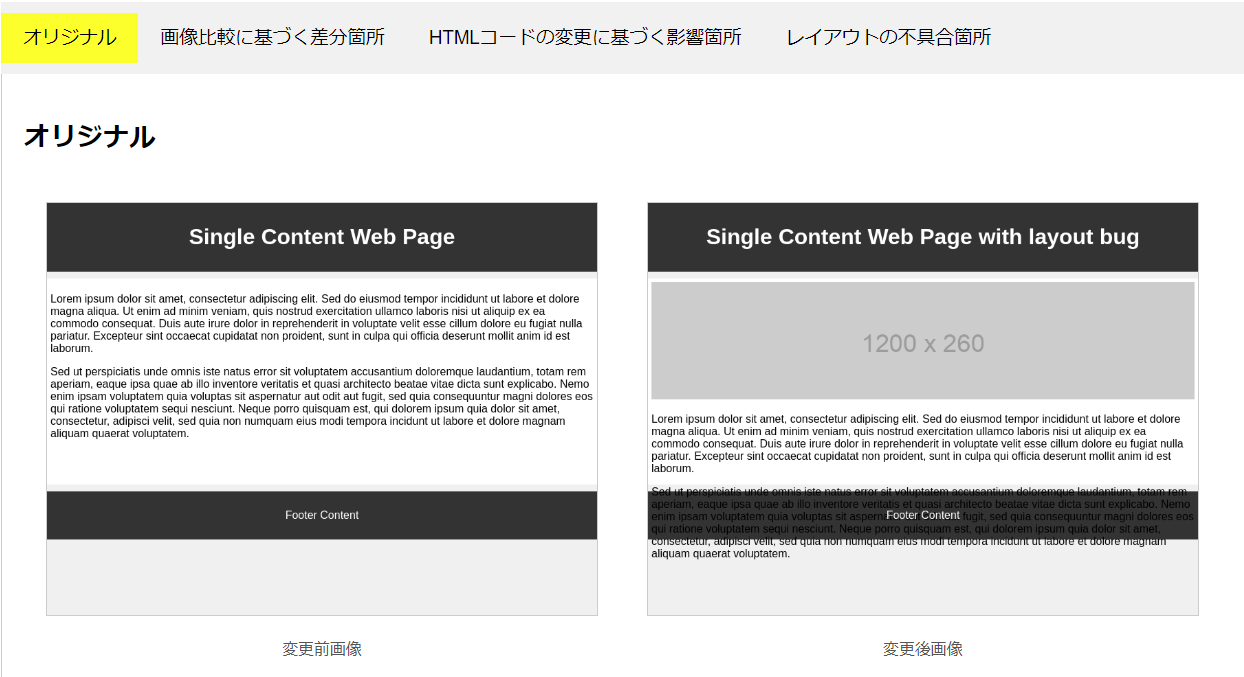
\includegraphics[width=1.0\columnwidth]{image/5/ex3_original.png}
        \caption{画面要素の重なりを埋め込んだWebページの変更前画像と変更後画像}
        \label{fig: ex3_original}
    \end{center}
\end{figure}
\begin{figure}[tp]
    \begin{center}
        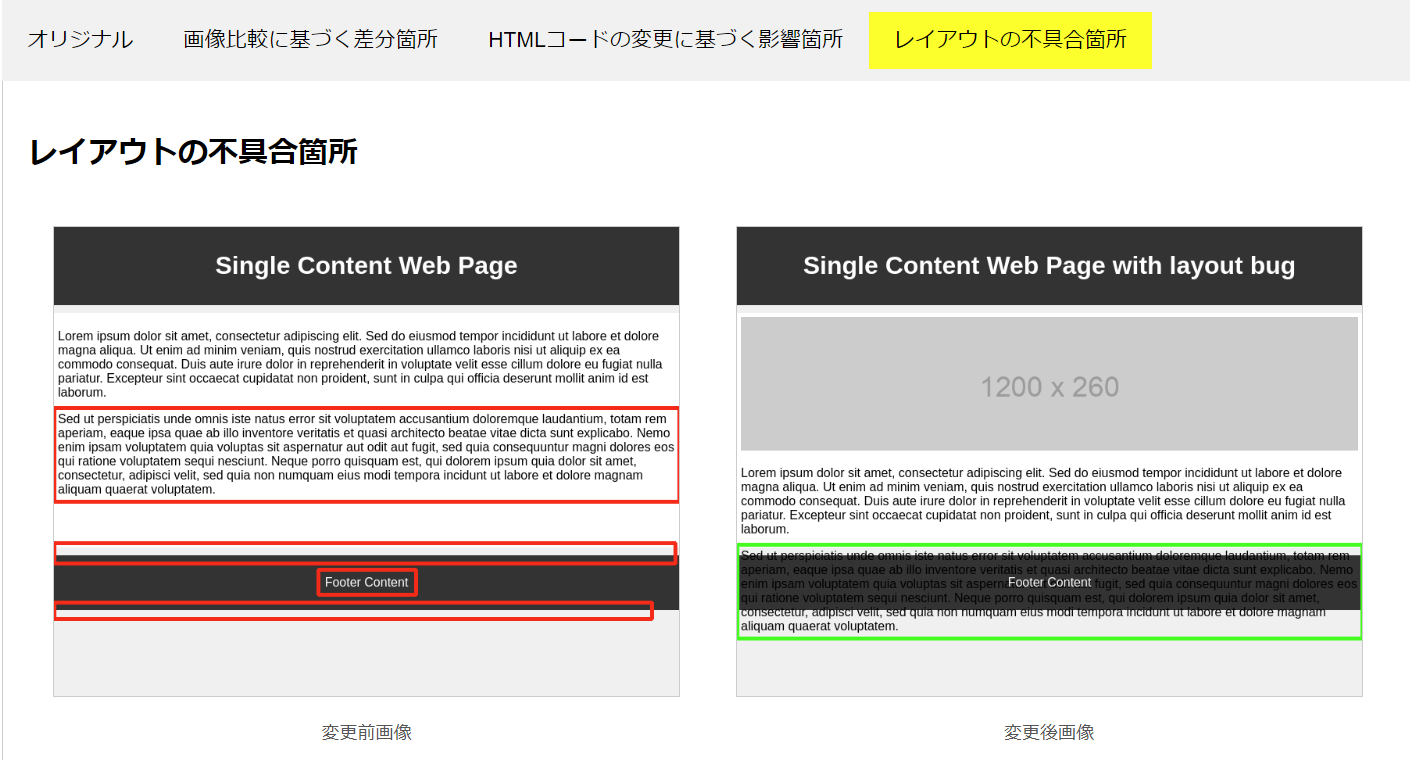
\includegraphics[width=1.0\columnwidth]{image/5/ex3_subeffect.png}
        \caption{図\ref{fig: ex3_original}に対して画面要素の重なりを可視化した変更前画像と変更後画像}
        \label{fig: ex3_subeffect}
    \end{center}
\end{figure}
図\ref{fig: ex3_subeffect}を見ると、変更後画像上にテキストとフッターの2つの画面要素が緑枠内で重なっていることが確認できる。
また、変更前画像上には、先ほど述べたテキストとフッターが赤枠で囲まれていることから、それらの画面要素が重なってできた画面要素の重なりであると確認できる。
このことから、画面要素の重なりが発生していると判断できる。
\par
以上のことから、\toolName は、画面要素の重なりを可視化することを確認できた。


% \section{画面要素の隠れが発生したWebページ}\label{subsec:result_rect_area}
% \subsection{Case1:開発者の意図しないレイアウトの不具合}\label{subsec:result_rect_area}

% \subsection{Case2:開発者が意図して画面要素を消した場合}\label{subsec:result_underline_area}

% \subsection{Case3:開発者が意図せず画面要素を消した場合}\label{subsec:result_underline}


% \section{画面要素の見切れが発生したWebページ}\label{subsec:result_underline_area}
% \subsection{Case1:開発者の意図しないレイアウトの不具合}\label{subsec:result_rect_area}

% \subsection{Case2:開発者が意図して画面要素を消した場合}\label{subsec:result_underline_area}

% \subsection{Case3:開発者が意図せず画面要素を消した場合}\label{subsec:result_underline}

% \section{画面要素の重なりが発生したWebページ}\label{sec:result_area_detection}

% \subsection{Case1:開発者の意図しないレイアウトの不具合}\label{subsec:result_rect_area}

% \subsection{Case2:開発者が意図して画面要素を消した場合}\label{subsec:result_underline_area}

% \subsection{Case3:開発者が意図せず画面要素を消した場合}\label{subsec:result_underline}